\subsection{OpenMP directives and constructs}

\begin{frame}[fragile]{OpenMP Directives}

  \begin{block}{A legal OpenMP Directive must has the following format (C/C++):}
    \begin{tabular}{|c|c|c|c|}
      \hline
      Pragma       & Directive                       & [clause[ [,]clause] ... ] \\
      \hline
      \#pragma omp & parallel, atomic, critical, ... & 0 to many                 \\
      \hline
    \end{tabular}
  \end{block}
  \begin{itemize}
    \item \emoji{chestnut} \textbf{For example:}
          \vspace{-5pt}
          \begin{minted}[fontsize=\scriptsize]{c}
#pragma omp parallel for collapse(2) private(tmp_v, d, v)
    \end{minted}
    \item Case sensitive
    \item Affects the block (single statement or wrapped by \verb|{}|) after this directive
    \item \emoji{zany-face} Here's an official \href{https://www.openmp.org/wp-content/uploads/OpenMPRefCard-5-2-web.pdf}{\textbf{Cheet Sheet}}
  \end{itemize}
\end{frame}

\begin{frame}[fragile]{Constructs}
  \emoji{thinking} What is the difference between \textbf{construct} and \textbf{directive}?

  \emoji{nerd-face} An OpenMP construct is a formation for which the directive is executable.\footnote{https://www.openmp.org/spec-html/5.2/openmpse14.html}

  \begin{minted}[fontsize=\small,highlightlines={5},highlightcolor=Khaki1]{c}
#pragma omp parallel    // <--\--- Directive
{                       //     |
    printf("Do sth.");  //     | Construct
}                       // ---/
\end{minted}

\end{frame}

\begin{frame}{Work-distribution constructs}
  \begin{columns}[T]

    \begin{column}{0.7\textwidth}
      \begin{figure}
        \centering
        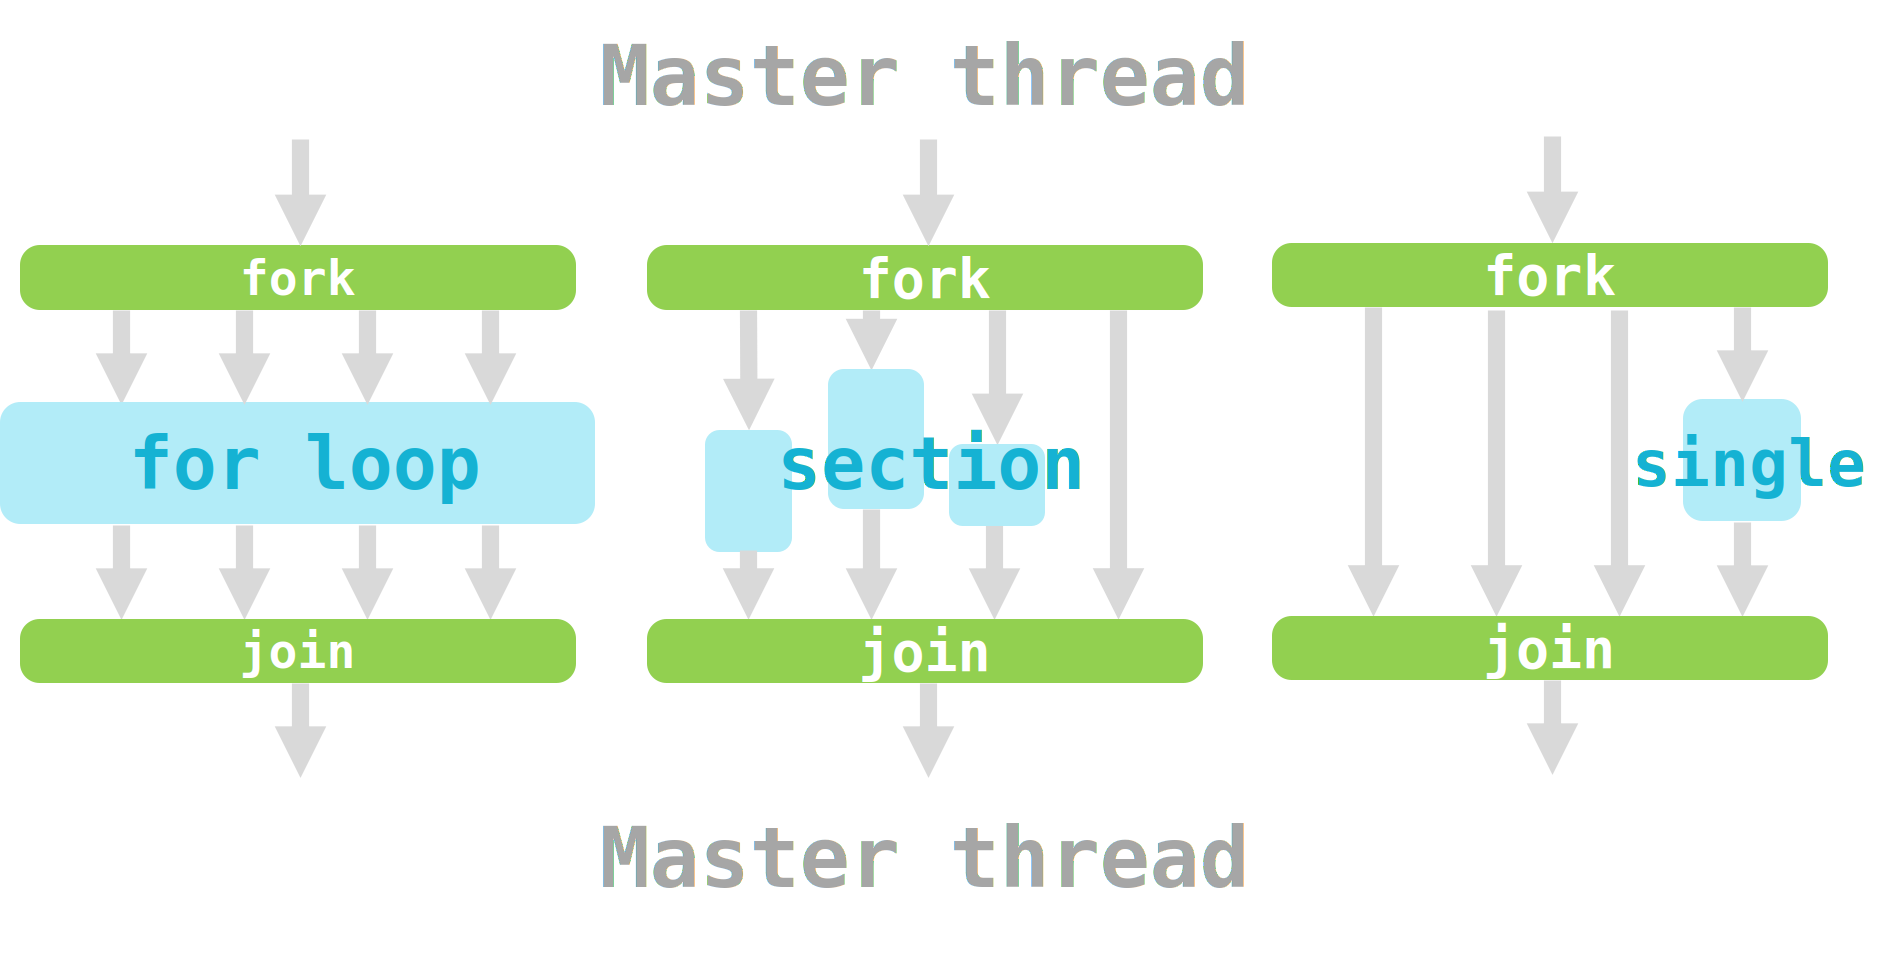
\includegraphics[width=1\linewidth]{day8_am/img/Work-distribution.png}
      \end{figure}
    \end{column}

    \begin{column}{0.3\textwidth}
      \vspace{2em}
      Work-distribution constructs:
      \begin{itemize}
        \item \textbf<1>{single}
        \item \textbf<2>{section}
        \item \textbf<3>{for}
      \end{itemize}
    \end{column}

  \end{columns}
\end{frame}

\begin{frame}[fragile]{\textit{parallel} Directive}
  \vspace{-10pt} % Align minted to the top
  \begin{minted}[fontsize=\small,highlightlines={5},highlightcolor=Khaki1]{c}
#include <stdio.h>
#include <omp.h>
int main() {
  printf("Welcome to OpenMP!\n");
  #pragma omp parallel
  {
    int ID = omp_get_thread_num();
    printf("hello(%d)", ID);
    printf("world(%d)\n", ID);
  }
  printf("Bye!");
  return 0;
}
      \end{minted}
\end{frame}

\begin{frame}[fragile]{Combined Constructs and Directives}
  \textbf{Example 2: \textit{parallel for} Directive}
  \begin{columns}[T] % align columns at top
    \begin{column}{0.5\textwidth}
      \vspace{-10pt} % Align minted to the top
      \begin{minted}[fontsize=\scriptsize]{c}
// Addition of two vectors
for (int i = 0; i < N; i++) {
    c[i] = a[i] + b[i];
}
      \end{minted}
    \end{column}

    \begin{column}{0.5\textwidth}
      \vspace{-10pt} % Align minted to the top
      \begin{minted}[fontsize=\scriptsize, highlightlines={2}]{c}
// Addition of two vectors
#pragma omp parallel for
for (int i = 0; i < N; i++) {
    c[i] = a[i] + b[i];
}
      \end{minted}
    \end{column}
  \end{columns}
  \begin{figure}
    \centering
    \includegraphics<1-2>[width=0.55\linewidth]{day8_am/img/parallel-for-1.png}
  \end{figure}
  \centering \uncover<2>{\emoji{exploding-head} Not 4x speed up}

  \uncover<3>{\emoji{hugging-face} \textbf{Overhead}: any combination of excess or indirect computation time, memory, bandwidth, or other resources that are required to perform a specific task.}
\end{frame}

\begin{frame}[fragile]{Loop Schedule}


  \begin{minted}[fontsize=\scriptsize]{c}
#pragma omp parallel for
for (int i = 0; i < N; i++) {
    c[i] = f(i); // What if f is not O(1)
}
\end{minted}

  Workload is unbalanced!

\end{frame}

\begin{frame}[fragile]{Loop Schedule}
  \begin{figure}
    \centering
    \includegraphics[width=0.8\linewidth]{day8_am/img/schedule-trace.png}
  \end{figure}

  \centering
  Static, Dynamic, Guided, Runtime, Auto

\end{frame}

\begin{frame}[fragile]{Loop Schedule - Static}

  \begin{minted}[fontsize=\scriptsize]{c}
#pragma omp parallel for schedule(static)
for (int i = 0; i < N; i++) {
    c[i] = f(i);
}
\end{minted}

  Static, Dynamic, Guided, Auto
\end{frame}

\begin{frame}[fragile]{Loop Schedule - Dynamic}

  \begin{minted}[fontsize=\scriptsize]{c}
#pragma omp parallel for schedule(dynamic, 2)
for (int i = 0; i < N; i++) {
    c[i] = f(i); // What is f is O(N^2)
}
\end{minted}

  \begin{itemize}
    \item[\emoji{thumbs-up}] Pros: More flexible scheduling
    \item[\emoji{thumbs-down}] Cons: More overhead in scheduling
  \end{itemize}

\end{frame}

\begin{frame}[fragile]{Nested \textit{for} Loop}
  \begin{columns}[T] % align columns at top
    \begin{column}{0.5\textwidth}
      \vspace{-10pt} % Align minted to the top
      \begin{minted}[fontsize=\scriptsize]{c}
// Matrix Element-wise Addition
#pragma omp parallel for
for (int i = 0; i < n; i++) {
    for (int j = 0; j < n; j++) {
        c[i][j] = a[i][j] + b[i][j];
    }
}
      \end{minted}
    \end{column}

    \begin{column}{0.5\textwidth}
      \vspace{-10pt} % Align minted to the top
      \begin{minted}[fontsize=\scriptsize, highlightlines={1}]{c}
#pragma omp parallel for collapse(2)
for (int i = 0; i < n; i++) {
    for (int j = 0; j < n; j++) {
        c[i][j] = a[i][j] + b[i][j];
    }
}
      \end{minted}
    \end{column}
  \end{columns}
\end{frame}